% \documentclass[titlepage, a4paper]{mwart}
%\documentclass[aps,prl,showpacs,10pt,superscriptaddress,nidanfloat,twocolumn,% draft]{revtex4-1}
\documentclass{article}
\usepackage[margin=0.8in]{geometry}
\usepackage{amsmath,amsfonts,amssymb,amsthm}
\usepackage{graphicx, setspace}
\usepackage{authblk}
\usepackage{mathtools}
\usepackage[export]{adjustbox}
\usepackage{placeins}
\let\Oldsection\section
\renewcommand{\section}{\FloatBarrier\Oldsection}
\let\Oldsubsection\subsection
\renewcommand{\subsection}{\FloatBarrier\Oldsubsection}
\let\Oldsubsubsection\subsubsection
\renewcommand{\subsubsection}{\FloatBarrier\Oldsubsubsection}

\usepackage[utf8]{inputenc}
\usepackage[T1]{fontenc}
\usepackage[english,polish]{babel}
\usepackage{breqn} %break long equations, use dmath instead of equation
\newtheorem{theorem}{Theorem}[section]
\newtheorem{example}{Example}[section]
\newtheorem{exercise}{Exercise}[section]
\newtheorem{solution}[exercise]{Solution}
\newtheorem{corollary}{Corollary}[theorem]
\newtheorem{lemma}[theorem]{Lemma}
\newtheorem{definition}{Definition}[section]
\newtheorem{axiom}{Axiom}[section]
\newtheorem*{remark}{Remark}
\newtheorem*{comment}{Comment}
\newtheorem{question}{Question}[section]
% \usepackage{polski}
\linespread{1.15}
\usepackage[pdftex,colorlinks=true,citecolor=blue,linkcolor=magenta]{hyperref}
\usepackage[backend=bibtex,sorting=none]{biblatex}
\bibliography{Mechanics}

% \usepackage[backend=bibtex]{biblatex}
% \addbibresource[location=remote]{http://127.0.0.1:23119/better-bibtex/collection?/1/.biblatex}
% \makeatletter
% \newcommand{\labeltext}[3][]{%
%     \@bsphack%
%     \csname phantomsection\endcsname% in case hyperref is used
%     \def\tst{#1}%
%     \def\labelmarkup{\emph}% How to markup the label itself
% %\def\refmarkup{\labelmarkup}% How to markup the reference
%     \def\refmarkup{}%
%     \ifx\tst\empty\def\@currentlabel{\refmarkup{#2}}{\label{#3}}%
%     \else\def\@currentlabel{\refmarkup{#1}}{\label{#3}}\fi%
%     \@esphack%
%     \labelmarkup{#2}% visible printed text.
% }
% \makeatother
\title{Classical Mechanics}
\author[1]{Ranza}\affil[1]{ScienceNotebooks GitHub rep}

\renewcommand\Affilfont{\itshape\small}
\begin{document}
\selectlanguage{english}
\maketitle

\section{Principle of least action}

Given the Lagrangian \(L\) of variables \(q_i,\dot{q}_i\) the principle of least action states

\begin{equation}\begin{aligned}\frac{\partial L}{\partial q_i}-\partial _t\frac{\partial L}{\partial \dot{q}}=0\end{aligned} \label{LeastAction}\end{equation}

Equation~\ref{LeastAction} can be found in~\cite{arnold1989mathematical}

\begin{remark}Variable which doesn’t occur in the Lagrangian is called cyclic and is connected with a conserved quantity (symmetry).\end{remark}

\section{Another section}

\begin{figure}[!htb]\centering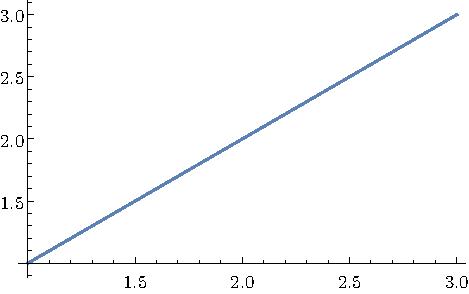
\includegraphics[scale=0.7,max width=\textwidth]{plotName.pdf}\caption{ This is a \(TEX\) exportable plot, tagged automatically }\label{plotName}\end{figure} 

which means that you can reference it from text (example fig.~\ref{plotName}) the same way as equations.
\appto{\bibsetup}{\raggedright} %For keeping the bib within margins
\printbibliography
\end{document}